\section{Hasil dan Pembahasan}
\label{sec:hasildanpembahasan}

Dilakukan pengujian dan analisis terhadap perancangan dan implementasi yang telah di desain sebelumnya. Pengujian yang dilakukan meliputi pengujian Sensor Load Cell terhadap Robot dan Sistem Keseimbangan Robot. 

\begin{enumerate}[label=\Alph*.]

    \item Pengujian Karakterisasi Pada Masing-Masing Sensor Load Cell
    \label{subsec:hasil-pembahasan-karakterisasi}

        \hspace*{1em} Pengujian kalibrasi sensor load cell dilakukan dengan menggunakan lima bandul referensi massa (50g, 100g, 200g, 500g, dan 1000g). Bandul terkecil (50 gram) digunakan untuk menentukan koefisien gradien, sedangkan konstanta diperoleh dari \textit{tare weight} (titik 0 ketika \emph{load cell} tidak ada beban). Data hasil perhitungan ini kemudian digunakan untuk menghitung tingkat kesalahan (\textit{error}) dari setiap \emph{load cell} yang digunakan dengan membandingkan dengan massa aktual. 

        \begin{table}[h]
            \centering
            \caption{Hasil Karakterisasi Load Cell Pertama}
            \begin{tabular}{|c|c|c|}
                \hline
                \textbf{Berat Aktual (gr)} & \textbf{Load Cell 1 Pembacaan (gr)} & \textbf{Error (gr)} \\
                \hline
                50    & 50    & 0   \\
                100   & 101   & 1   \\
                200   & 202   & 2   \\
                500   & 505   & 5   \\
                1000  & 1004  & 4   \\
                \hline
            \end{tabular}
            \label{tab:Kalibrasi_Load_Cell_1}
        \end{table}

        \begin{table}[h]
            \centering
            \caption{Hasil Karakterisasi Load Cell Kedua}
            \begin{tabular}{|c|c|c|}
                \hline
                \textbf{Berat Aktual (gr)} & \textbf{Load Cell 2 Pembacaan (gr)} & \textbf{Error (gr)} \\
                \hline
                50        & 50        & 0   \\
                100       & 100       & 0   \\
                200       & 200       & 0   \\
                500       & 500       & 0   \\
                1000      & 994       & 6   \\           
                \hline
        \end{tabular}
        \label{tab:Kalibrasi_Load_Cell_2}
        \end{table}

        \begin{table}[h]
            \centering
            \caption{Hasil Karakterisasi Load Cell Ketiga}
            \begin{tabular}{|c|c|c|}
                \hline
                \textbf{Berat Aktual (gr)} & \textbf{Load Cell 3 Pembacaan (gr)} & \textbf{Error (gr)} \\
                \hline
                50        & 50        & 0    \\    
                100       & 103       & 3    \\    
                200       & 203       & 3    \\    
                500       & 494       & 6    \\    
                1000      & 981       & 19   \\               
                \hline
        \end{tabular}
        \label{tab:Kalibrasi_Load_Cell_3}
        \end{table}

        \begin{table}[h]
            \centering
            \caption{Hasil Karakterisasi Load Cell Keempat}
            \begin{tabular}{|c|c|c|}
                \hline
                \textbf{Berat Aktual (gr)} & \textbf{Load Cell 4 Pembacaan (gr)} & \textbf{Error (gr)} \\
                \hline
                50        & 50        & 0   \\     
                100       & 97        & 3   \\     
                200       & 204       & 4   \\     
                500       & 500       & 0   \\     
                1000      & 1003      & 3   \\                
                \hline
        \end{tabular}
        \label{tab:Kalibrasi_Load_Cell_4}
        \end{table}
    
        
        \hspace*{1em} Hasil pengujian karakterisasi pada masing-masing \emph{load cell} menunjukkan adanya kesalahan pengukuran yang bervariasi, berkisar antara 0 hingga 19 gram. Kesalahan ini tidak linear, menunjukkan bahwa kesalahan pengukuran tidak konstan pada setiap \emph{load cell}. Meskipun demikian, persamaan linear masih dapat digunakan untuk menghitung massa aktual dari pembacaan \emph{load cell} meskipun tidak sepenuhnya akurat.

    \item Pengujian Tekanan Pada Telapak Kaki
    \label{subsec:hasil-pembahasan-tekanan}

        \hspace*{1em} Pengujian ini dilakukan untuk mendapatkan data tekanan yang dihasilkan oleh kaki kanan dan kaki kiri ketika diberikan beban secara merata. Data tekanan yang dihasilkan oleh kaki kanan dan kaki kiri dapat dilihat pada Tabel \ref{tab:pengukuran_berat_kaki_kiri} dan Tabel \ref{tab:pengukuran_berat_kaki_kanan}.

        \begin{table}[h!]
            \centering
            \caption{Tabel Pembacaan Tekanan untuk Kaki Kiri}
            \begin{tabular}{|c|c|c|}
                \hline
                \textbf{Berat Aktual (gr)} & \textbf{Pembacaan (gr)} & \textbf{Error (gr)} \\
                \hline
                50    & 52    & 2   \\
                100   & 110   & 10  \\
                200   & 220   & 20  \\
                300   & 304   & 4   \\
                500   & 512   & 12  \\
                700   & 701   & 1   \\
                1000  & 1050  & 50  \\
                1300  & 1325  & 25  \\
                1500  & 1512  & 12  \\
                1800  & 1788  & 12  \\
                \hline
                \textbf{Rata-rata Error (gr)} & \multicolumn{2}{c|}{\textbf{14.8}} \\
                \hline
            \end{tabular}
            \label{tab:pengukuran_berat_kaki_kiri}
        \end{table}

        \begin{table}[h!]
            \centering
            \caption{Tabel Pembacaan Tekanan untuk Kaki Kanan}
            \begin{tabular}{|c|c|c|}
                \hline
                \textbf{Berat Aktual (gr)} & \textbf{Pembacaan (gr)} & \textbf{Error (gr)} \\
                \hline
                50    & 46    & 4    \\
                100   & 98    & 2    \\
                200   & 215   & 15   \\
                300   & 325   & 25   \\
                500   & 505   & 5    \\
                700   & 722   & 22   \\
                1000  & 1025  & 25   \\
                1300  & 1347  & 47   \\
                1500  & 1500  & 0    \\
                1800  & 1819  & 19   \\
                \hline
                \textbf{Rata-rata Error (gr)} & \multicolumn{2}{c|}{\textbf{16.4}} \\
                \hline
            \end{tabular}
            \label{tab:pengukuran_berat_kaki_kanan}
        \end{table}

        \begin{figure}[h]
            \centering
            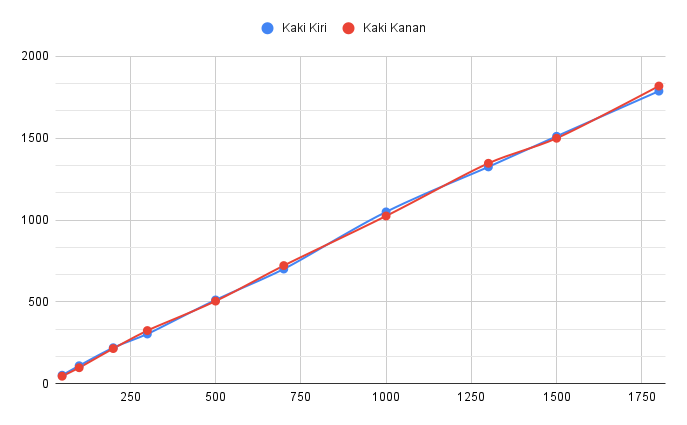
\includegraphics[width=0.4\textwidth]{gambar/chart_tekanan_kaki.png}
            \caption{Grafik Hubungan Antara Berat Aktual dan Pembacaan \emph{Load Cell} pada Kaki Kiri dan Kaki Kanan}
            \label{fig:tekanan_kaki}
        \end{figure}

        \hspace*{1em} Hasil pengukuran tekanan pada kaki kiri dan kaki kanan menunjukkan bahwa pembacaan \emph{load cell} pada kedua kaki memiliki kesalahan yang bervariasi, berkisar antara 0 hingga 50 gr. Kesalahan ini disebabkan oleh perbedaan karakteristik antara \emph{load cell} pada kaki kiri dan kaki kanan. Pada Gambar \ref{fig:tekanan_kaki} terlihat bahwa grafik tekanan yang dihasilkan oleh kaki kanan dan kaki kiri memiliki nilai pembacaan yang serupa.

    \newpage

    \item Pengujian Pusat Tekanan Terhadap Robot
    \label{subsec:hasil-pembahasan-pusat-tekanan}

        \hspace*{1em} Pengujian ini dilakukan ketika robot menjalankan motion dan mengambil data input dari sensor load cell dengan interval 50 ms. Tujuan pengujian ini adalah untuk mendapatkan data pusat tekanan saat robot menjalankan motion. Pengujian dilakukan seperti pada Gambar \ref{fig:pusat_tekanan_robot} dengan mengambil 3 data pusat tekanan saat robot melakukan motion berjalan di tempat yaitu ketika robot pada posisi \textit{double support}, mengangkat kaki kanan, dan mengangkat kaki kiri. 

        \begin{figure}[h]
            \centering
            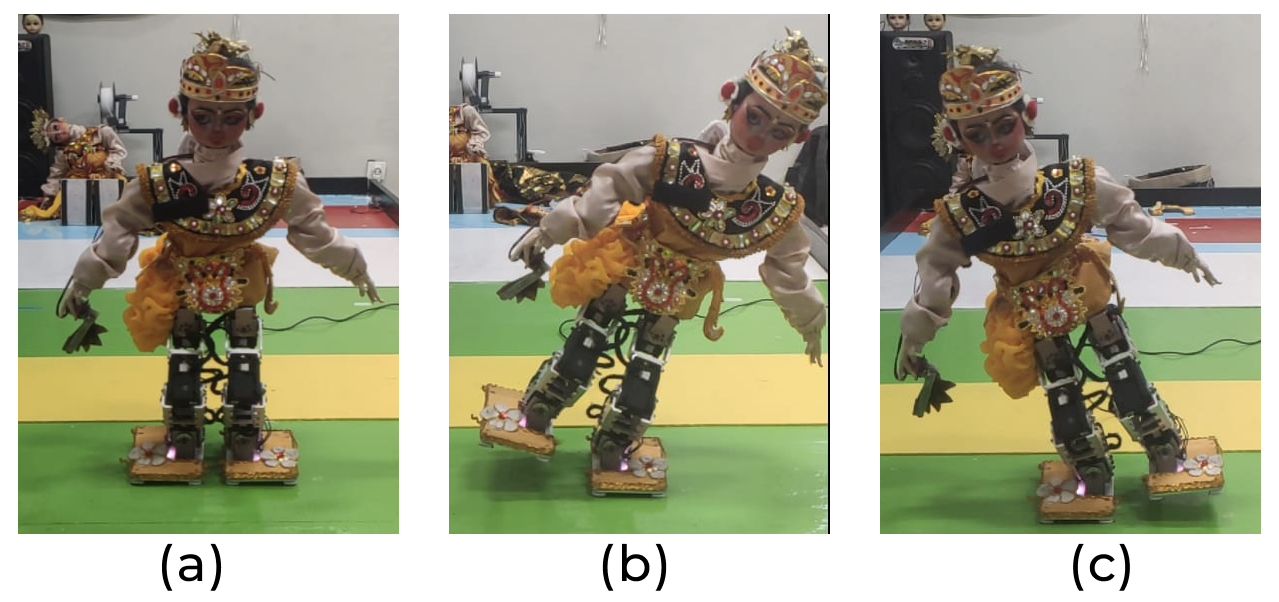
\includegraphics[width=0.4\textwidth]{gambar/hasil/jalan_ditempat.png}
            \caption{Postur Robot Saat Berjalan di Tempat \\ (a)  \textit{Double Phase Support} \\ (b)  Mengangkat Kaki Kanan \\ (c)  Mengangkat Kaki Kiri}
            \label{fig:pusat_tekanan_robot}
        \end{figure}

        \hspace*{1em} Untuk menampilkan data pusat tekanan yang dihasilkan oleh robot, digunakan visualisasi kaki robot. Posisi pusat tekanan pada sumbu X dan Y ditampilkan dalam bentuk titik koordinat dengan skala 2:1. Visualisasi ini dapat membantu dalam memahami posisi pusat tekanan pada robot ketika melakukan gerakan berjalan di tempat. Data diambil berdasarkan 3 data pusat tekanan yang dihasilkan pada skenario sebelumnya.

        \hspace*{1em} Pada Gambar \ref{fig:pusat_tekanan_robot_double} pusat tekanan pada Sumbu X 0.09 pada dan pada Sumbu Y 0.01. Pada Gambar \ref{fig:pusat_tekanan_robot_angkat_kiri} pusat tekanan pada Sumbu X -1.30 dan pada Sumbu Y 0.16. Sedangkan pada Gambar \ref{fig:pusat_tekanan_robot_angkat_kanan} pusat tekanan pada Sumbu X 1.44 dan Sumbu Y 0.03. Dari hasil visualisasi ini, pusat tekanan pada sumbu X mengalami perubahan yang signifikan ketika robot mengangkat kaki kiri dan kaki kanan, sedangkan pada sumbu Y, titik koordinat pusat tekanan tetap berada di tengah-tengah telapak kaki.
        
        \newpage

        \begin{figure}[h]
            \centering
            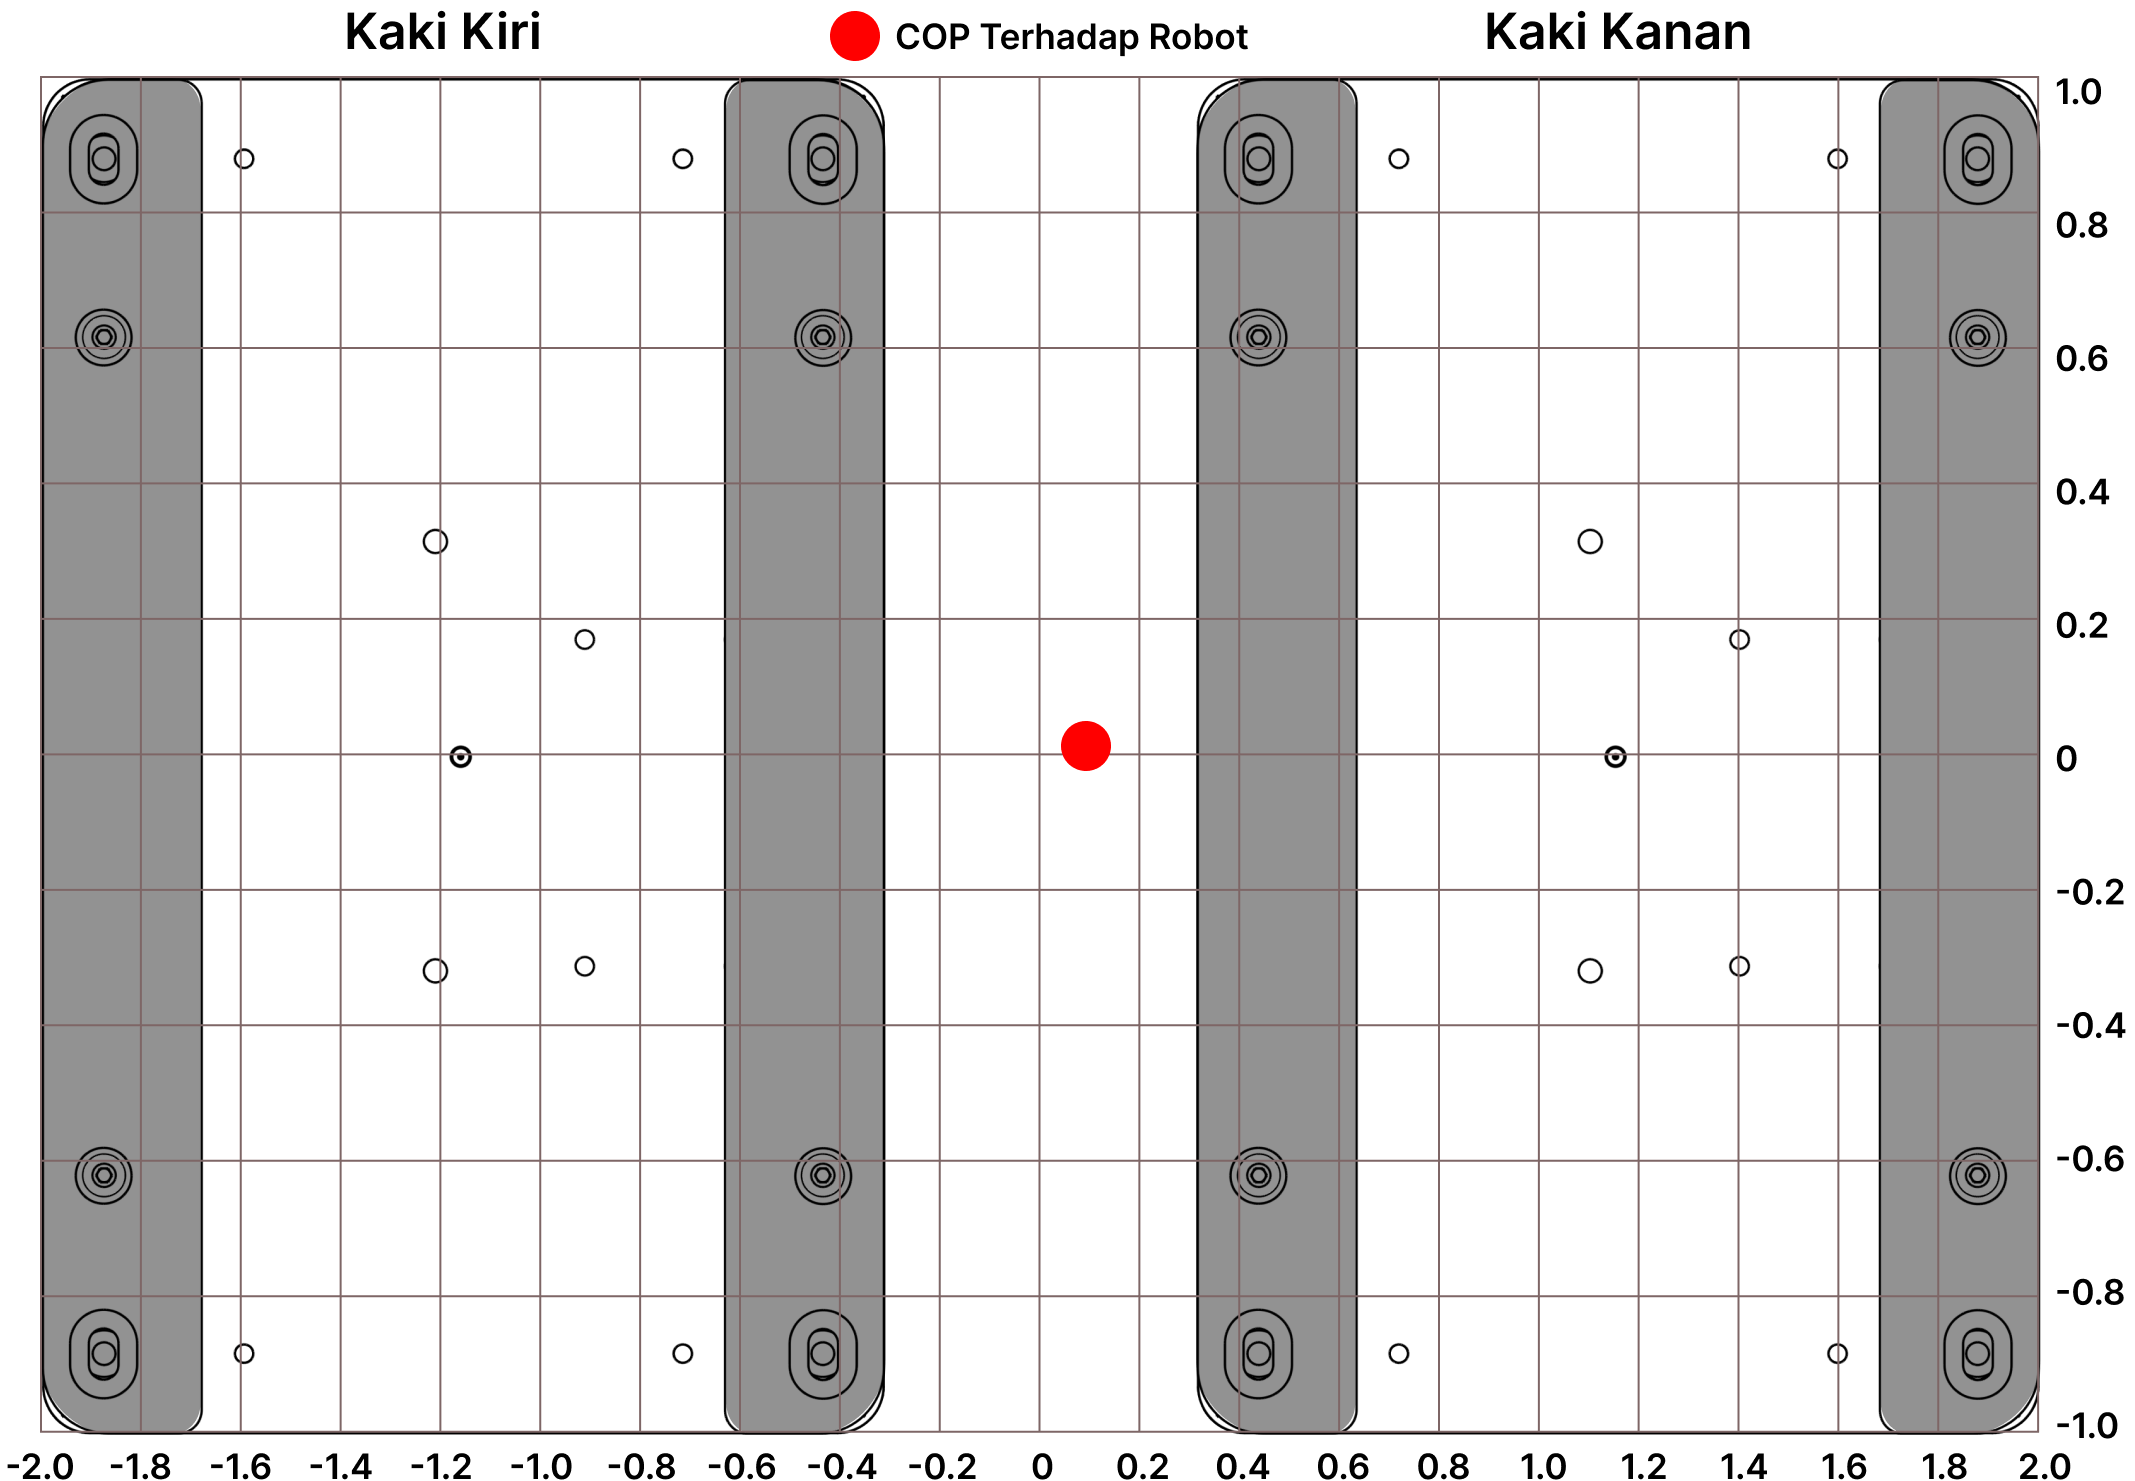
\includegraphics[width=0.3\textwidth]{gambar/hasil/cop_double_phase.png}
            \caption{\textit{COP} Robot Ketika \textit{Double Phase Support}}
            \label{fig:pusat_tekanan_robot_double}
        \end{figure}
        
        \begin{figure}[h]
            \centering
            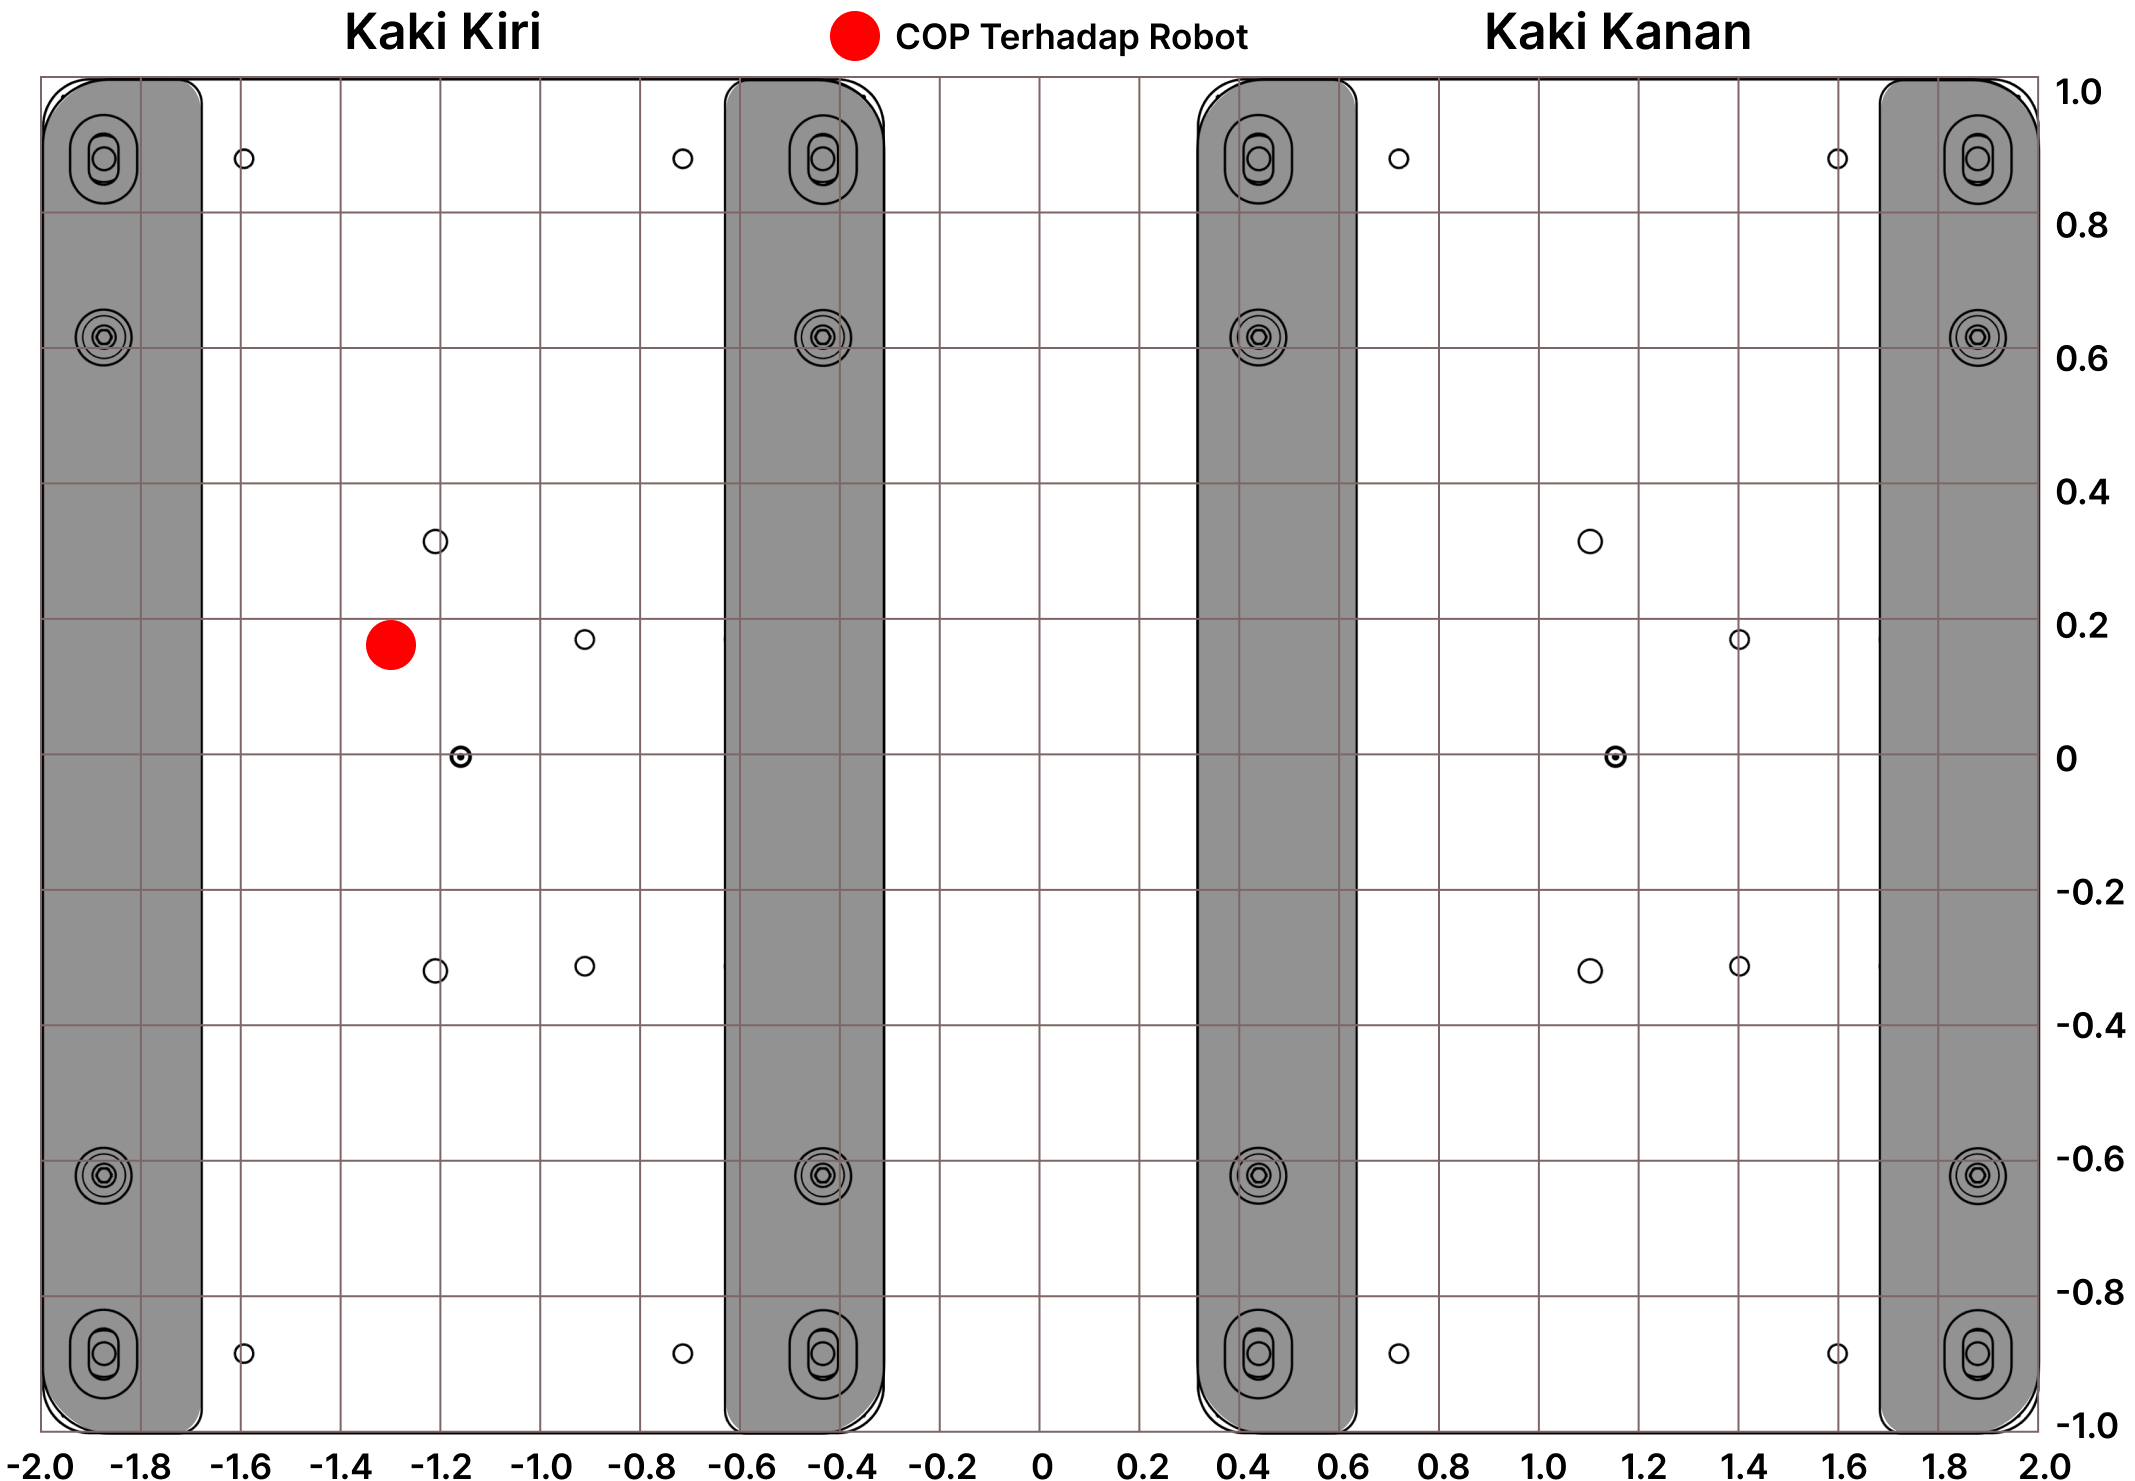
\includegraphics[width=0.3\textwidth]{gambar/hasil/cop_angkat_kiri.png}
            \caption{\textit{COP} Robot Ketika Robot Mengangkat Kaki Kiri}
            \label{fig:pusat_tekanan_robot_angkat_kiri}
        \end{figure}
        
        \begin{figure}[h]
            \centering
            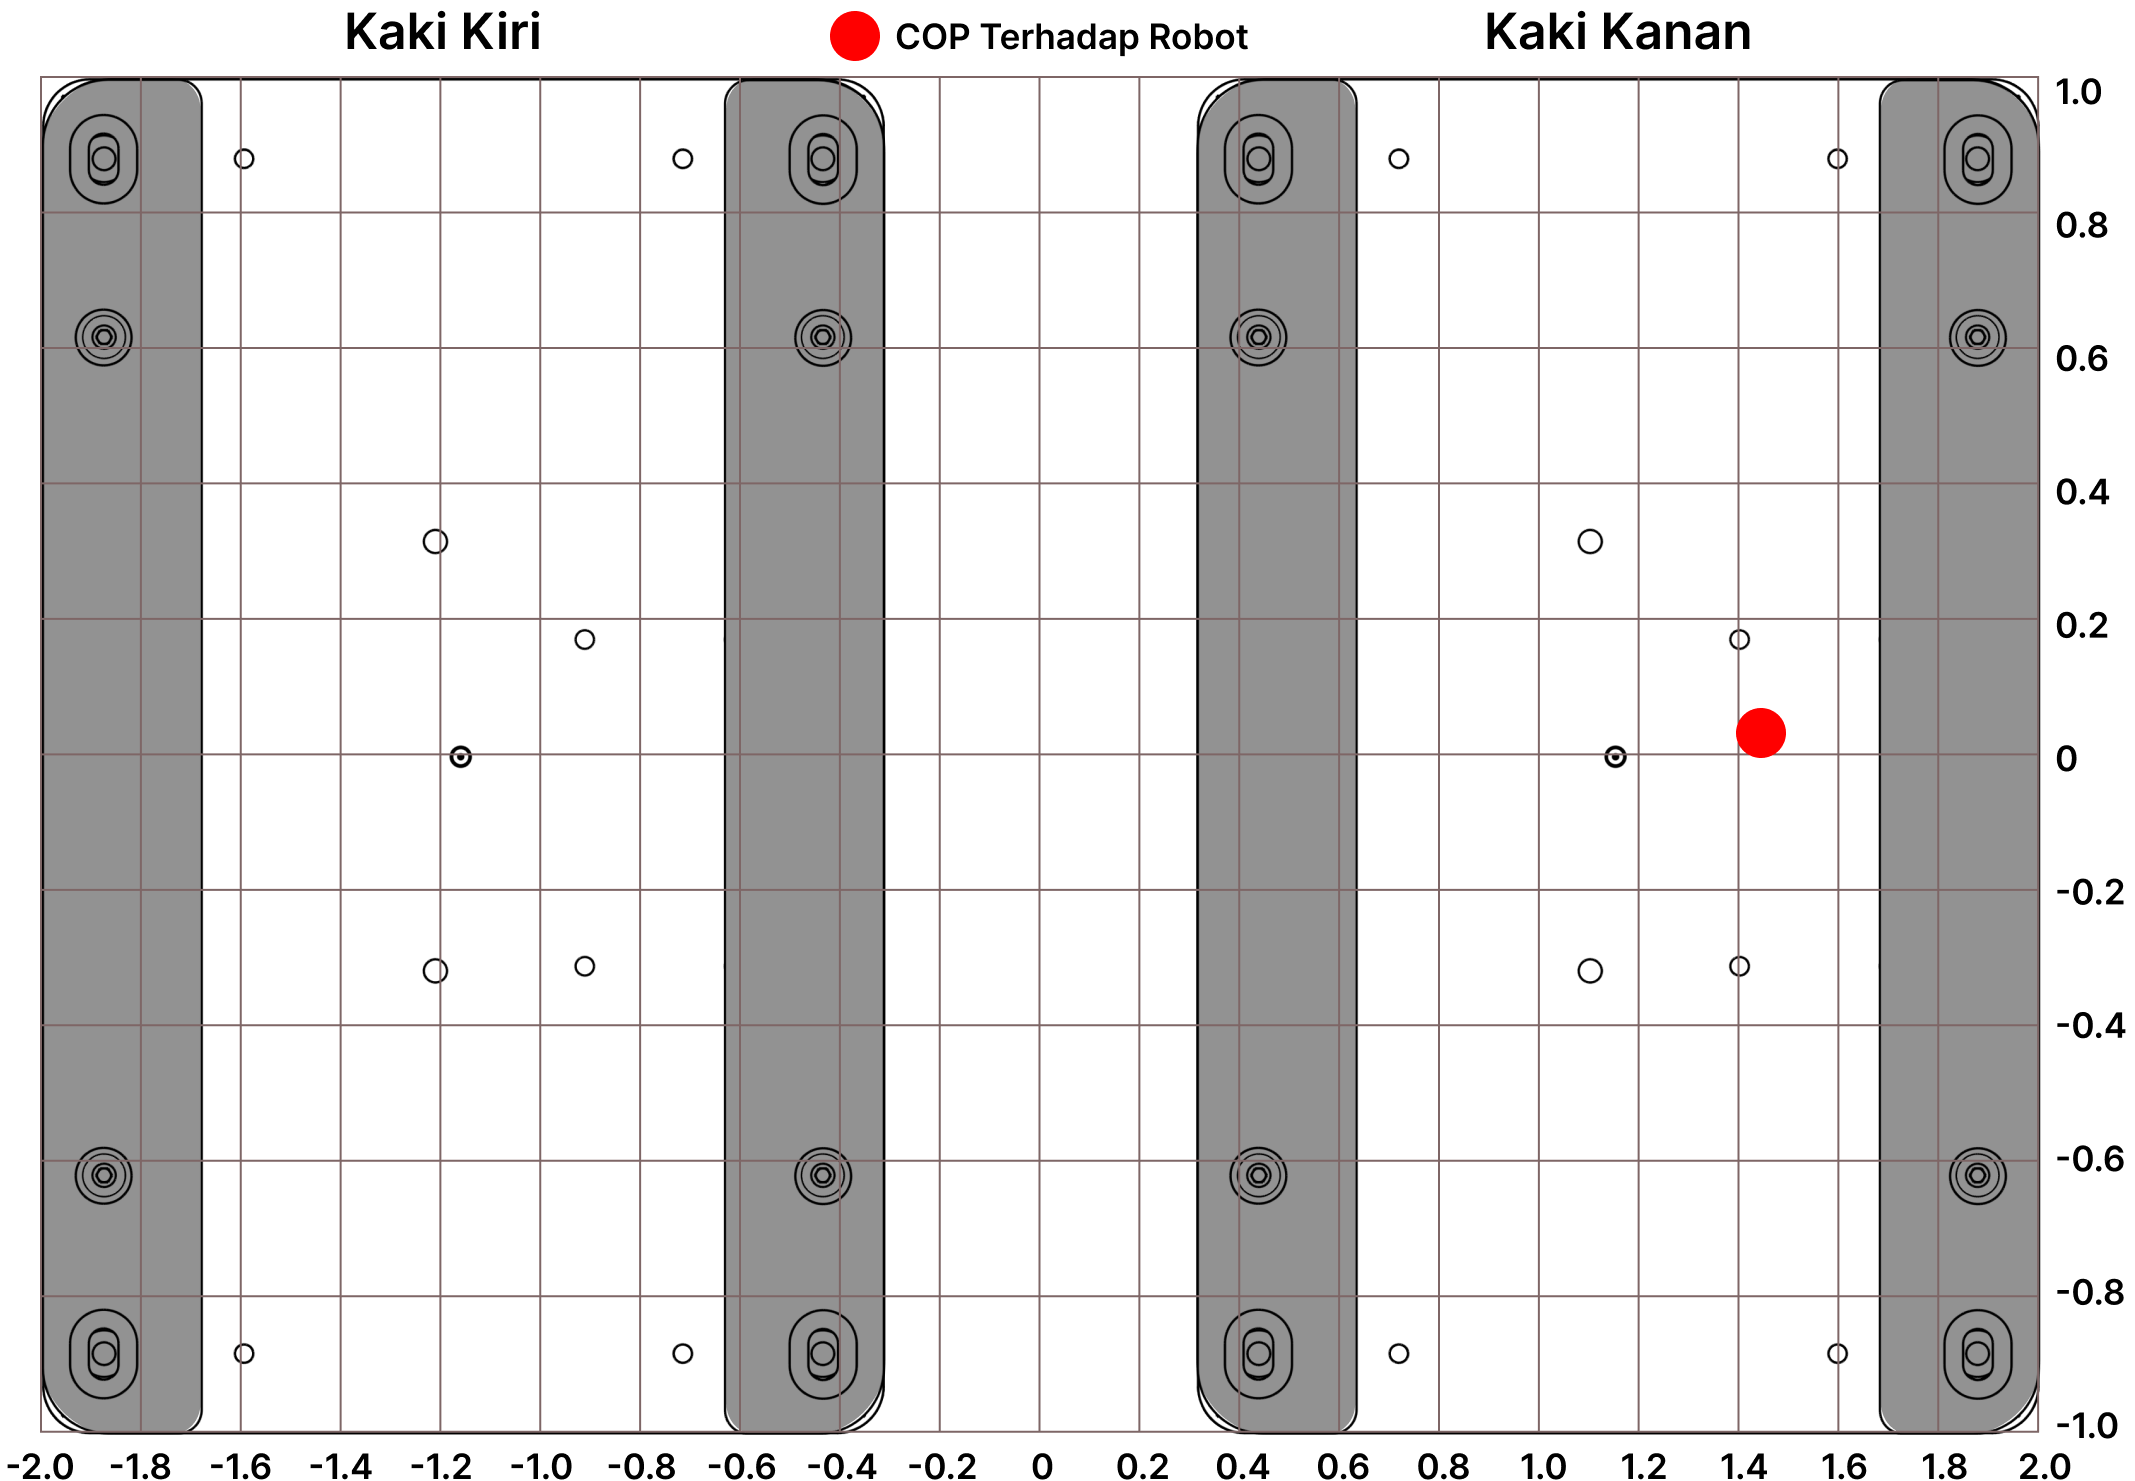
\includegraphics[width=0.3\textwidth]{gambar/hasil/cop_angkat_kanan.png}
            \caption{\textit{COP} Robot Ketika Robot Mengangkat Kaki Kanan}
            \label{fig:pusat_tekanan_robot_angkat_kanan}
        \end{figure}
        

    \item Pengujian Sistem Kontrol PID
    \label{subsec:hasil-pembahasan-pid}

        \hspace*{1em} Pada pengujian ini, dilakukan pengujian sistem keseimbangan robot dengan kontrol PID. Hasil yang akan dianalisis adalah respons sistem ketika menggunakan sistem kontrol PID dan tanpa kontrol PID. Pengujian dilakukan dengan mengangkat kaki kanan atau kaki kiri dengan kemiringan 3 derajat.

        \hspace*{1em} Gambar \ref{fig:robot_not_fall} merupakan hasil pengujian robot sudah menggunakan kontroler PID. Sedangkan Gambar \ref{fig:robot_fall} tanpa kontroler PID. Pada Gambar \ref{fig:robot_not_fall}, jika nilai pusat tekanan pada sumbu X melebihi batas maksimum dalam waktu tertentu, maka robot akan terjatuh. Hal ini menunjukkan bahwa nilai \emph{error} yang dihasilkan oleh kontroler PID tidak dapat dikalkulasi dengan baik karena nilai input yang diterima oleh kontroler PID tidak sesuai dengan yang diharapkan.

        \newpage

        
        \begin{figure}[h]
            \centering
            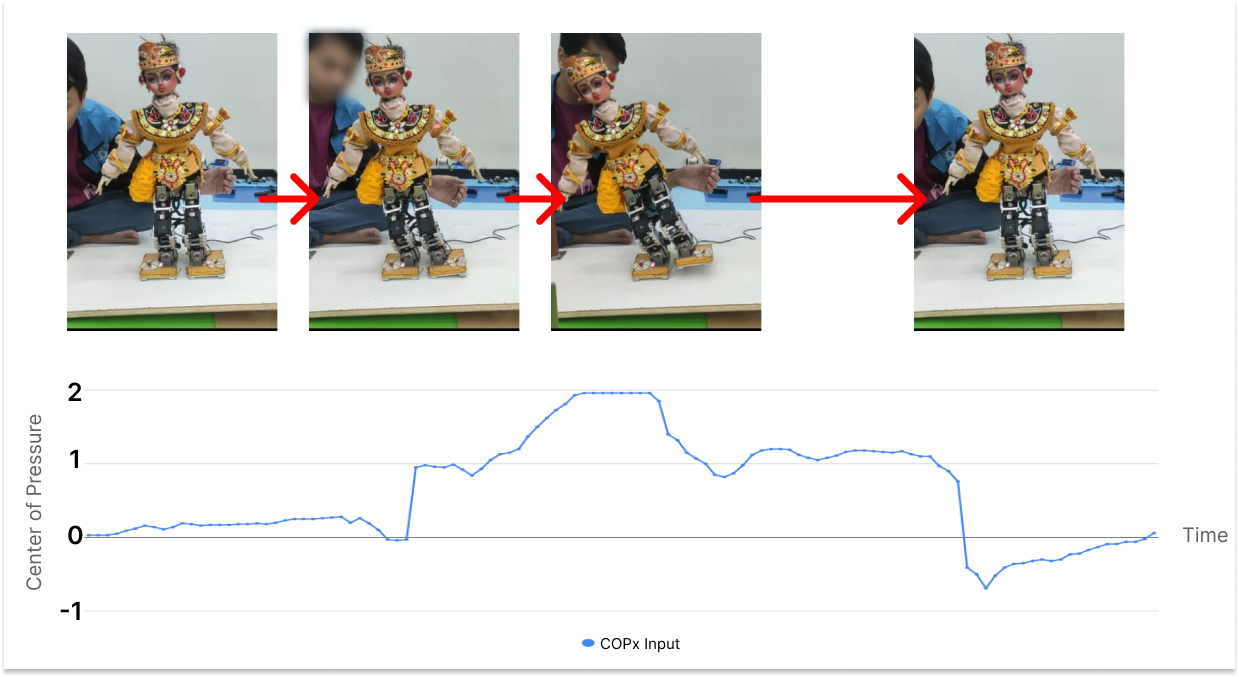
\includegraphics[width=0.4\textwidth]{gambar/hasil/hasil_pid.png}
            \caption{Grafik Respon Sistem Dengan Kontrol PID (Tidak Jatuh)}
            \label{fig:robot_not_fall}
        \end{figure}


        \begin{figure}[h]
            \centering
            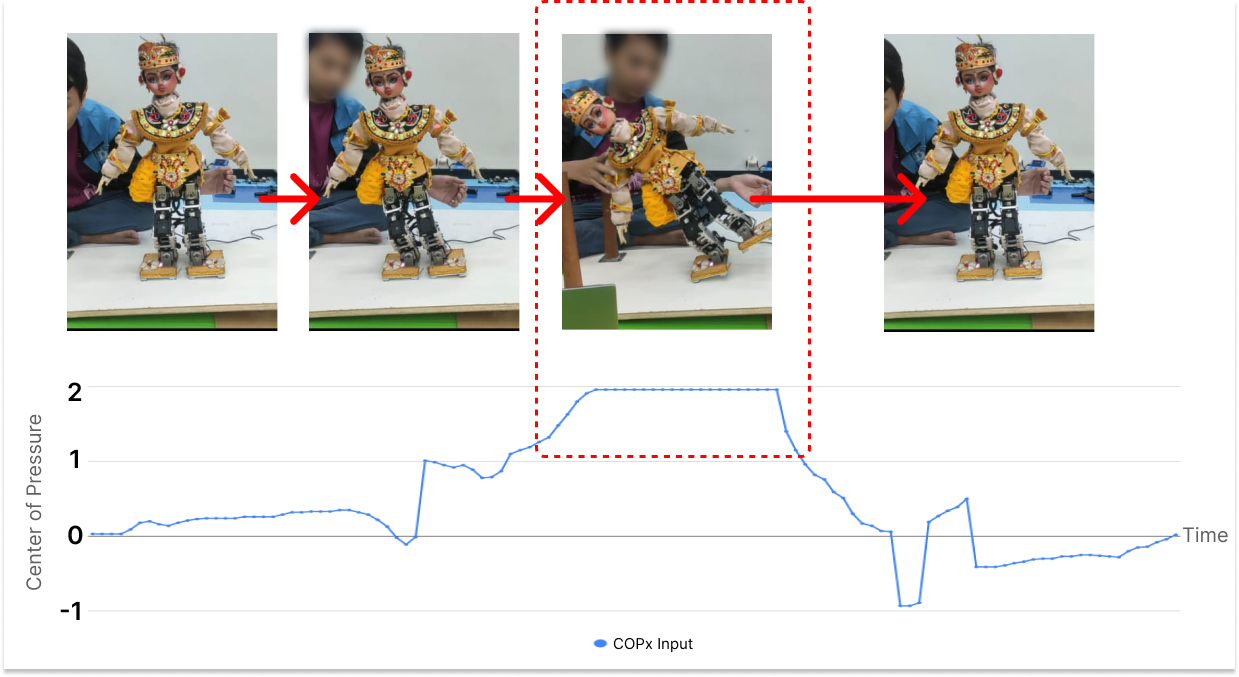
\includegraphics[width=0.4\textwidth]{gambar/hasil/hasil_no_pid.png}
            \caption{Grafik Respon Sistem Tanpa Kontrol PID (Jatuh)}
            \label{fig:robot_fall}
        \end{figure}

    \item Pengujian Pengaruh Parameter PID
    \label{subsec:hasil-pembahasan-parameter-pid}
        
        \hspace*{1em} Pengujian ini, dilakukan skenario pengujian ini meliputi analisis pengaruh masing-masing parameter PID. Hasil yang akan dianalisis adalah pengaruh parameter PID terhadap respon sistem dan hasil nilai \textit{Root Mean Square (RMS)} yang dihasilkan oleh sistem. Pengujian dilakukan sama seperti pada pengujian sebelumnya, yaitu mengangkat kaki kanan atau kaki kiri dengan kemiringan 3 derajat.

        \begin{table}[h]
            \centering
            \caption{Hasil Pengujian Pengaruh Parameter P, Mengangkat Kaki Kiri Dengan Kemiringan 3 Derajat}
            \begin{tabular}{|c|c|c|c|c|}
                \hline
                \textbf{PID} & \textbf{Fall} & \textbf{Not Fall} & \textbf{Success} & RMS Error \\
                \hline
                $K_p = 0.00$ & 6 & 0 & 0   \% & 0.7598 \\
                $K_p = 0.05$ & 6 & 0 & 0   \% & 0.7690 \\
                $K_p = 0.10$ & 0 & 6 & 100 \% & 0.7779 \\
                $K_p = 0.15$ & 1 & 5 & 83  \% & 0.8145 \\
                $K_p = 0.20$ & 1 & 5 & 83  \% & 0.8870 \\
                $K_p = 0.25$ & 0 & 6 & 100 \% & 0.8801 \\            
                \hline
            \end{tabular}
            \label{tab:pengujian_p}
        \end{table}

        \hspace*{1em} Hasil pengujian pada Tabel \ref{tab:pengujian_p} menunjukkan bahwa nilai optimal parameter Kp untuk menjaga keseimbangan robot berkisar antara 0.10 hingga 0.20. Pada Kp = 0.00 dan Kp = 0.05, semua pengujian gagal dengan robot selalu jatuh. Nilai Kp = 0.10 menunjukkan performa terbaik dengan keberhasilan 100\% dalam menjaga keseimbangan pada gerakan mengangkat kaki kanan dan kiri di kemiringan 3 derajat. Nilai Kp yang lebih tinggi, seperti Kp = 0.25, menunjukkan penurunan performa. Hasil \textit{Root Mean Square} (RMS) menunjukkan error terkecil pada Kp = 0.10 dengan nilai 0.7779, menegaskan pentingnya pengaturan Kp yang tepat untuk stabilitas robot.

        \begin{table}[h]
            \centering
            \caption{Hasil Pengujian Pengaruh Parameter PI, Mengangkat Kaki Kanan Dengan Kemiringan 3 Derajat}
            \begin{tabular}{|c|c|c|c|c|}
                \hline
                \textbf{PID} & \textbf{Fall} & \textbf{Not Fall} & \textbf{Success} & RMS Error \\
                \hline
                $K_p = 0.1, K_i = 0.01$ & 2 & 4 & 66 \%  & 0.9701\\
                $K_p = 0.1, K_i = 0.02$ & 2 & 4 & 66 \%  & 0.8950\\
                $K_p = 0.1, K_i = 0.04$ & 1 & 5 & 83 \%  & 0.9345\\
                $K_p = 0.1, K_i = 0.10$ & 0 & 6 & 100 \% & 0.8471\\
                $K_p = 0.1, K_i = 0.20$ & 0 & 6 & 100 \% & 0.8980\\           
                \hline
            \end{tabular}
            \label{tab:pengujian_pi}
        \end{table}

        \hspace*{1em} Hasil pengujian pada Tabel \ref{tab:pengujian_pi} menunjukkan bahwa nilai optimal parameter Ki untuk menjaga keseimbangan robot berkisar antara 0.10 hingga 0.20. Pada Ki = 0.01 dan Ki = 0.02  robot gagal menjaga keseimbangan dengan tingkat keberhasilan 66\% hingga 83\%. Sebaliknya, pada Ki = 0.10 dan Ki = 0.20  robot berhasil menjaga keseimbangan dengan tingkat keberhasilan 100\% pada gerakan mengangkat kaki kanan dan kiri di kemiringan 3 derajat. Hasil \textit{Root Mean Square} (RMS) menunjukkan nilai terendah pada Ki = 0.10 sebesar 0.8471, sementara nilai tertinggi pada Ki = 0.01 sebesar 0.9701. Pengaruh Ki terhadap performa tidak terlalu signifikan, dan dalam beberapa kasus, nilai Ki yang lebih tinggi menurunkan performa sistem, menunjukkan bahwa parameter Ki dalam kontrol PID pada sistem ini tidak terlalu diperlukan.

        \begin{table}[h]
            \centering
            \caption{Hasil Pengujian Pengaruh Parameter PD, Mengangkat Kaki Kanan Dengan Kemiringan 3 Derajat}
            \begin{tabular}{|c|c|c|c|c|}
                \hline
                \textbf{PID} & \textbf{Fall} & \textbf{Not Fall} & \textbf{Success} & RMS Error \\
                \hline
                $K_p = 0.1, K_d = 0.005$ & 0 & 6 & 100 \% & 0.7143 \\
                $K_p = 0.1, K_d = 0.010$ & 0 & 6 & 100 \% & 0.7077 \\
                $K_p = 0.1, K_d = 0.020$ & 2 & 4 & 66  \% & 0.7262 \\
                $K_p = 0.1, K_d = 0.050$ & 5 & 1 & 16  \% & 0.7344 \\
                $K_p = 0.1, K_d = 0.100$ & 6 & 0 & 0   \% & 0.9231 \\          
                \hline
            \end{tabular}
            \label{tab:pengujian_pd}
        \end{table}

        \hspace*{1em} Hasil pengujian pada Tabel \ref{tab:pengujian_pd} menunjukkan bahwa nilai optimal parameter Kd untuk menjaga keseimbangan robot berkisar antara 0.005 hingga 0.020. Pada Kd = 0.005 dan Kd = 0.010, robot berhasil menjaga keseimbangan dengan tingkat keberhasilan 100\%. Namun, pada Kd = 0.020, tingkat keberhasilan menurun menjadi 66\%, dan pada Kd = 0.050, tingkat keberhasilan hanya 16\%. Pada Kd = 0.100, robot selalu jatuh. Hasil \textit{Root Mean Square} (RMS) menunjukkan nilai terendah pada Kd = 0.010 sebesar 0.7077, sementara nilai tertinggi pada Kd = 0.100 sebesar 0.9231. Pengaruh Kd terhadap performa sistem cukup signifikan, dan nilai Kd yang lebih tinggi menurunkan performa sistem.

\end{enumerate}